O Transmissor/Receptor Assíncrono Universal (\emph{Universal Asynchronous Receiver/Transmitter}, UART), é um periférico de transmissão e recepção de dados usado na comunicação entre dispositivos, sendo esta comunicação realizada de forma serial e assíncrona, ou seja sem a necessidade de transmissão do sinal de clock de referência. Este modo de transmissão faz necessário o uso de apenas duas vias de comunicação uma para a transmissão e outra para a recepção de dados.

\section{Padrão da Comunicação}

\begin{figure}[H]
\centering
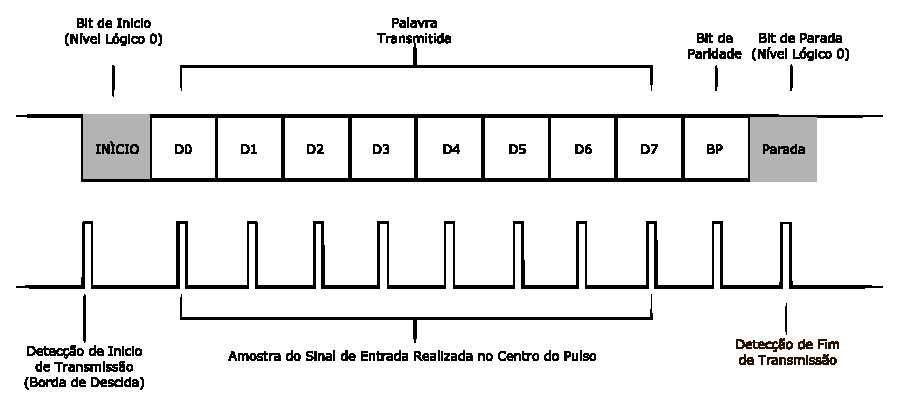
\includegraphics[width=1\textwidth] {figuras/uart.eps}
    \caption{Protocolo de envio na comunicação UART}
    \label{fig:uart}
\end{figure}

Para que a comunicação UART seja realizada é necessário que o sinal de transmissão obedeça a um protocolo. Quando uma palavra é transmitida, primeiro é enviado um bit de início de transmissão para o receptor. Este bit deve ser de nível logico 0 para que a ocorrência da borda de descida sinalize ao receptor que sincronize a amostragem do sinal a ser lido de modo que ela ocorra no meio de cada período de transmissão.  Após transmitir os dados é necessário enviar um bit informando a existência de paridade ou não, e por último é enviado um bit de nível lógico alto para informar o fim da transmissão. Esta sintaxe pode ser observada na figura \ref{fig:uart}.

\section{UART do TM4C1294NCPDT}


O Tiva TM4C1294NCPDT possui 8 módulos de comunicação UART. Cada um destes  possuem um gerador de \emph{baud-rate}, ou taxa de transmissão, que possibilitam  transmissões de até 7,5 Mbps em modo de normal transmissão e  15 Mbps em modo \emph{High Speed}. 

Para que seja possível regular o \emph{baud-rate} de forma mais precisa os módulos UART possuem um divisor de 22 bits, sendo 16 bits inteiros e 6 bits fracionários, pelo qual o módulo determina o período de transmissão de bit.

Já o buffer de leitura e transmissão do UART no Tiva tem um tamanho de 8 bits, porém para cada módulo existe uma FIFO de 16x8 bits tanto para transmissão quanto para recepção, sendo que o \emph{trigger} de interrupção de estouro da FIFO é selecionável entre 1/8, 1/4, 1/2, 3/4, 7/8 ou 8/8. 

O sinal de transmissão criado pelo UART do tiva pode transmitir dados seriais de 5,6,7 ou 8 bits de dados precedidos do bit de \emph{Start} e acompanhados de um bit de paridade, se estiver habilitado, e 1 ou 2 bits de parada. A figura \ref{fig:uartTiva} apresenta o sinal característico da transmissão UART do Tiva. 

\begin{figure}[H]
	\centering
	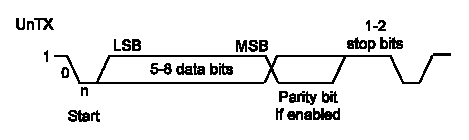
\includegraphics[width=0.5\textwidth] {figuras/uartTiva.eps}
	\caption{Sinal de Transmissão UART no Tiva TM4C1294NCPDT}
	\label{fig:uartTiva}
\end{figure}

A figura \ref{tab:CanaisUART} apresenta os pinos de entrada e saída do UART que podem ser usados no Tiva TM4C1294NCPDT.
  
\begin{table}[H]
	\centering
	\caption{Canais do UART - Tiva TM4C1294NCPDT \cite{DATASHEET_TIVA} }
	\label{tab:CanaisUART}
	\begin{tabular}{|c|c|c|c|l|}
		\rowcolor[HTML]{000000} 
		{\color[HTML]{FFFFFF} Pino}  & {\color[HTML]{FFFFFF} Mux/Função} & {\color[HTML]{FFFFFF} Tipo} & {\color[HTML]{FFFFFF} Buffer} & {\color[HTML]{FFFFFF} Descrição}  \\
		\hline
		UORx  & PA0 (1) & I & TTL & UART Módulo 0, recepção do sinal   \\
		\hline
		U0Tx  & PA1 (1) & O & TTL & UART Módulo 0, transmissão do sinal  \\
		U1Rx  & PB0 (1) & I & TTL & UART Módulo 1, recepção do sinal   \\
		      & PQ4 (1) &   &     &                                     \\
		\hline
		U1Tx  & PB1 (1) & O & TTL & UART Módulo 1, transmissão do sinal  \\
		\hline
		U2Rx  & PA6 (1) & I & TTL & UART Módulo 2, recepção do sinal   \\
		      & PD4 (1) &   &     &                                      \\
		\hline
		U2Tx  & PA7 (1) & O & TTL & UART Módulo 2, transmissão do sinal  \\
		      & PD5 (1) &   &     &                                      \\
		\hline
		U3Rx  & PA4 (1) (1) & I & TTL & UART Módulo 3, recepção do sinal   \\
	 	      & PJ0 (1) &   &     &                                      \\
		\hline
		U3Tx  & PA5 (1) & O & TTL & UART Módulo 3, transmissão do sinal  \\
	 	      & PJ1 (1) &   &     &                                      \\
		\hline
		U4Rx  & PK0 (1) & I & TTL & UART Módulo 4, recepção do sinal   \\
		      & PA2 (1) &   &     &                                      \\
		\hline
		U4Tx  & PK1 (1) & O & TTL & UART Módulo 4, transmissão do sinal  \\
		      & PA3 (1) &   &     &                                      \\
		\hline
		U5Rx  & PC6 (1) & I & TTL & UART Módulo 5, recepção do sinal\\
		\hline
		U5Tx  & PC7 (1) & O & TTL & UART Módulo 5, transmissão do sinal \\
		\hline
		U6Rx  & PP0 (1) & I & TTL & UART Módulo 6, recepção do sinal \\
		\hline
		U6Tx  & PP1 (1) & O & TTL & UART Módulo 6, transmissão do sinal\\
		\hline
		U7Rx  & PC4 (1) & I & TTL & UART Módulo 7, recepção do sinal \\
		\hline
		U7Tx  & PC5 (1) & O & TTL & UART Módulo 7, transmissão do sinal\\
		\hline
	\end{tabular}
\end{table}


\section{Na TivaWare}

As principais funções para o uso da comunicação UART na TivaWare são apresentadas nesta seção.

\begin{lstlisting}[style=funcao]
	void UARTClockSourceSet(uint32_t ui32Base,
							uint32_t ui32Source);
\end{lstlisting}

Configura a fonte de clock utilizada no barramento UART.

\begin{description}
	\item [\ttbu{ui32Base}]\hfill \\
	Base da UART a ser configurada. Normalmente \textbf{UART\emph{k}\_BASE}, onde \textbf{\emph{k}} é o número que identifica a base que está sendo configurada.
	
	\item [\ttbu{ui32Source}]\hfill \\
	Fonte de clock do UART.
	\begin{description}
		\item [\textbf{UART\_CLOCK\_SYSTEM}] clock fornecido pelo clock do sistema
		\item [\textbf{UART\_CLOCK\_PIOSC}] clock fornecido pelo oscilador interno de precisão
	\end{description}
\end{description}

\begin{lstlisting}[style=funcao]
	void UARTConfigSetExpClk(uint32_t ui32Base,
							 uint32_t ui32UARTClk,
							 uint32_t ui32Baud,
							 uint32_t ui32Config)
\end{lstlisting}

Configura os parâmetros da comunicação UART.

\begin{description}
	\item [\ttbu{ui32Base}]\hfill \\
	Base da UART a ser configurada. Normalmente \textbf{UART\emph{k}\_BASE}, onde \textbf{\emph{k}} é o número que identifica a base que está sendo configurada.
	
	\item [\ttbu{ui32UARTClk}]\hfill \\
	Valor do clock a ser configurado no periférico da UART.
	
	\item [\ttbu{ui32Baud}]\hfill \\
	Baud rate da comunicação UART.
	
	\item [\ttbu{ui32Config}]\hfill \\
	Valor formado pela operação OU lógica de 3 parâmetros: número de bits de dados, número de bits de parada e a paridade.
	
	\begin{description}
		\item [\textbf{UART\_CONFIG\_WLEN\_\emph{k}}] protocolo com \textbf{\emph{k}} bits de dados. Onde \textbf{\emph{k}} pode assumir os valores: 5, 6, 7 e 8
		\item [\textbf{UART\_CONFIG\_STOP\_\emph{k}}] define 1 ou 2 bits de parada. Sendo que \textbf{\emph{k}} assume os valores \textbf{ONE} ou \textbf{TWO}, respectivamente.
		\item [\textbf{UART\_CONFIG\_PAR\_\emph{k}}] onde \textbf{\emph{k}} pode assumir os valores:
		\begin{itemize}
			\item \textbf{NONE} sem bit de paridade
			\item \textbf{EVEN} com bit de paridade par
			\item \textbf{ODD} com bit de paridade ímpar
			\item \textbf{ONE} bit de paridade é sempre 1
			\item \textbf{ZERO} bit de paridade é sempre 0
		\end{itemize}

	\end{description}
\end{description}

\begin{lstlisting}[style=funcao]
	void UARTEnable(uint32_t ui32Base)
\end{lstlisting}

Habilita o funcionamento da comunicação UART.

\begin{description}
	\item [\ttbu{ui32Base}]\hfill \\
	Base da UART a ser habilitada. Normalmente \textbf{UART\emph{k}\_BASE}, onde \textbf{\emph{k}} é o número que identifica a base que está sendo configurada.
\end{description}

\begin{lstlisting}[style=funcao]
	void UARTDisable(uint32_t ui32Base)
\end{lstlisting}

Desabilita o funcionamento da comunicação UART.

\begin{description}
	\item [\ttbu{ui32Base}]\hfill \\
	Base da UART a ser desabilitada. Normalmente \textbf{UART\emph{k}\_BASE}, onde \textbf{\emph{k}} é o número que identifica a base que está sendo configurada.
\end{description}

\begin{lstlisting}[style=funcao]
	int32_t UARTCharGet(uint32_t ui32Base)
\end{lstlisting}

Pega próximo caractere recebido pela UART. Se não houver nada para ser lido, o programa trava e espera até haver um caractere.

\begin{description}
	\item [\ttbu{ui32Base}]\hfill \\
	Base da UART a ser lida. Normalmente \textbf{UART\emph{k}\_BASE}, onde \textbf{\emph{k}} é o número que identifica a base que está sendo configurada.
\end{description}

\begin{lstlisting}[style=funcao]
	int32_t UARTCharGetNonBlocking(uint32_t ui32Base)
\end{lstlisting}

Pega próximo caractere recebido pela UART. Se não houver nada para ser lido, a leitura é ignorada e o programa continua normalmente. Nesse caso, a função retorna -1.

\begin{description}
	\item [\ttbu{ui32Base}]\hfill \\
	Base da UART a ser lida. Normalmente \textbf{UART\emph{k}\_BASE}, onde \textbf{\emph{k}} é o número que identifica a base que está sendo configurada.
\end{description}

\begin{lstlisting}[style=funcao]
	void UARTCharPut(uint32_t ui32Base,
					 unsigned char ucData))
\end{lstlisting}

Envia um caractere para ser transmitido pela UART. Se não houver espaço na fila de transmissão, o programa é travado e aguarda até o caractere ser colocado na fila.

\begin{description}
	\item [\ttbu{ui32Base}]\hfill \\
	Base da UART a ser lida. Normalmente \textbf{UART\emph{k}\_BASE}, onde \textbf{\emph{k}} é o número que identifica a base que está sendo configurada.
	
	\item [\ttbu{ucData}]\hfill \\
	Caractere a ser transmitido pela UART.
\end{description}

\begin{lstlisting}[style=funcao]
	bool UARTCharPutNonBlocking(uint32_t ui32Base,
								unsigned char ucData))
\end{lstlisting}

Envia um caractere para ser transmitido pela UART. Se não houver espaço na fila de transmissão, a operação é ignorada e o programa continua normalmente. Nesse caso, a função retorna o valor \emph{false} e a operação deve ser repetida posteriormente.

\begin{description}
	\item [\ttbu{ui32Base}]\hfill \\
	Base da UART a ser lida. Normalmente \textbf{UART\emph{k}\_BASE}, onde \textbf{\emph{k}} é o número que identifica a base que está sendo configurada.
	
	\item [\ttbu{ucData}]\hfill \\
	Caractere a ser transmitido pela UART.
\end{description}

\begin{lstlisting}[style=funcao]
	bool UARTCharsAvail(uint32_t ui32Base)
\end{lstlisting}

Informa se há algum caractere para ser lido na fila de recepção.

\begin{description}
	\item [\ttbu{ui32Base}]\hfill \\
	Base da UART a ser lida. Normalmente \textbf{UART\emph{k}\_BASE}, onde \textbf{\emph{k}} é o número que identifica a base que está sendo configurada.
\end{description}

\begin{lstlisting}[style=funcao]
	bool UARTSpaceAvail(uint32_t ui32Base)
\end{lstlisting}

Informa se há espaço para ser enviado um novo byte para a fila de transmissão.

\begin{description}
	\item [\ttbu{ui32Base}]\hfill \\
	Base da UART a ser lida. Normalmente \textbf{UART\emph{k}\_BASE}, onde \textbf{\emph{k}} é o número que identifica a base que está sendo configurada.
\end{description}

\begin{lstlisting}[style=funcao]
	void UARTIntRegister(uint32_t ui32Port,
						 void (*pfnIntHandler)(void))
\end{lstlisting}

Configura a função de tratamento de uma interrupção da UART. Aquela que é chamada quando ocorre a interrupção.

\begin{description}
	\item [\ttbu{ui32Base}]\hfill \\
	Base da UART a ser configurada. Normalmente \textbf{UART\emph{k}\_BASE}, onde \textbf{\emph{k}} é o número que identifica a base que está sendo configurada.
	
	\item [\ttbu{pfnIntHandler}]\hfill \\
	Ponteiro da função de tratamento. Esta não deve receber nada como parâmetro e nem retornar nada.
\end{description}

\begin{lstlisting}[style=funcao]
	void UARTIntEnable(uint32_t ui32Base,
					   uint32_t ui32IntFlags)
\end{lstlisting}

Habilita as interrupções especificadas da UART especificada.

\begin{description}
	\item [\ttbu{ui32Base}]\hfill \\
	Base da UART a ser configurada. Normalmente \textbf{UART\emph{k}\_BASE}, onde \textbf{\emph{k}} é o número que identifica a base que está sendo configurada.
	
	\item [\ttbu{ui32IntFlags}]\hfill \\
	Pacote em formato de OU lógico com os parâmetros que especificam os eventos que podem causar a interrupção da UART. Cada parâmetro recebe uma definição no formato \textbf{UART\_INT\_\emph{k}}, onde \textbf{\emph{k}} é um valor entre os seguintes:
	\begin{itemize}
		\item \textbf{9BIT} interrupção por endereço de 9 bits
		\item \textbf{OE} interrupção por transbordo de fila
		\item \textbf{BE} interrupção por erro de parada
		\item \textbf{PE} interrupção por erro de paridade
		\item \textbf{FE} interrupção por erro de enquadramento
		\item \textbf{RT} interrupção por estouro de tempo de recepção
		\item \textbf{TX} interrupção por transmissão
		\item \textbf{RX} interrupção por recepção
		\item \textbf{DSR} interrupção por DSR
		\item \textbf{DCD} interrupção por DCD
		\item \textbf{CTS} interrupção por CTS
		\item \textbf{RI} interrupção por RI
	\end{itemize}
\end{description}

\begin{lstlisting}[style=funcao]
	void UARTIntDisable(uint32_t ui32Base,
					   uint32_t ui32IntFlags)
\end{lstlisting}

Desabilita as interrupções especificadas da UART especificada.

\begin{description}
	\item [\ttbu{ui32Base}]\hfill \\
	Base da UART a ser configurada. Normalmente \textbf{UART\emph{k}\_BASE}, onde \textbf{\emph{k}} é o número que identifica a base que está sendo configurada.
	
	\item [\ttbu{ui32IntFlags}]\hfill \\
	Pacote em formato de OU lógico com os parâmetros que especificam os eventos que podem causar a interrupção da UART. Cada parâmetro recebe uma definição no formato \textbf{UART\_INT\_\emph{k}}, onde \textbf{\emph{k}} é um valor entre os seguintes:
	\begin{itemize}
		\item \textbf{9BIT} interrupção por endereço de 9 bits
		\item \textbf{OE} interrupção por transbordo de fila
		\item \textbf{BE} interrupção por erro de parada
		\item \textbf{PE} interrupção por erro de paridade
		\item \textbf{FE} interrupção por erro de enquadramento
		\item \textbf{RT} interrupção por estouro de tempo de recepção
		\item \textbf{TX} interrupção por transmissão
		\item \textbf{RX} interrupção por recepção
		\item \textbf{DSR} interrupção por DSR
		\item \textbf{DCD} interrupção por DCD
		\item \textbf{CTS} interrupção por CTS
		\item \textbf{RI} interrupção por RI
	\end{itemize}
\end{description}

\begin{lstlisting}[style=funcao]
	void UARTIntClear(uint32_t ui32Base,
					   uint32_t ui32IntFlags)
\end{lstlisting}

Limpa a flag que armazena a ocorrência das interrupções especificadas da UART especificada.

\begin{description}
	\item [\ttbu{ui32Base}]\hfill \\
	Base da UART a ser configurada. Normalmente \textbf{UART\emph{k}\_BASE}, onde \textbf{\emph{k}} é o número que identifica a base que está sendo configurada.
	
	\item [\ttbu{ui32IntFlags}]\hfill \\
	Pacote em formato de OU lógico com os parâmetros que especificam as interrupção da UART a serem limpas. Cada parâmetro recebe uma definição no formato \textbf{UART\_INT\_\emph{k}}, onde \textbf{\emph{k}} é um valor entre os seguintes:
	\begin{itemize}
		\item \textbf{9BIT} interrupção por endereço de 9 bits
		\item \textbf{OE} interrupção por transbordo de fila
		\item \textbf{BE} interrupção por erro de parada
		\item \textbf{PE} interrupção por erro de paridade
		\item \textbf{FE} interrupção por erro de enquadramento
		\item \textbf{RT} interrupção por estouro de tempo de recepção
		\item \textbf{TX} interrupção por transmissão
		\item \textbf{RX} interrupção por recepção
		\item \textbf{DSR} interrupção por DSR
		\item \textbf{DCD} interrupção por DCD
		\item \textbf{CTS} interrupção por CTS
		\item \textbf{RI} interrupção por RI
	\end{itemize}
\end{description}

\section{Exemplo}

A seguir, é apresentado um exemplo de configuração da UART. Um exemplo mais abrangente pode ser visto na Seção \ref{sec:exUart}

\begin{lstlisting}[style=citacao]
	// Habilita GPIO A usado na comunicacao da UART 0
	MAP_SysCtlPeripheralEnable(SYSCTL_PERIPH_GPIOA);
	// Aguarda 3 SysCtlDelay
	// Aproximadamente 10 ciclos de clock
	MAP_SysCtlDelay(3);
	// Configura PA0 no modo Rx da UART 0
	MAP_GPIOPinConfigure(GPIO_PA0_U0RX);
	// Configura PA1 no modo Tx da UART 0
	MAP_GPIOPinConfigure(GPIO_PA1_U0TX);

	// Habilita UART 0
	MAP_SysCtlPeripheralEnable(SYSCTL_PERIPH_UART0);
	// Configura PA0 e PA1 como pinos de comunicacao da UART
	MAP_GPIOPinTypeUART(
		GPIO_PORTA_BASE, GPIO_PIN_0 | GPIO_PIN_1);
	// Configura UART 0
	// fonte de clock 120MHz para 115.200 baud 8N1
	UARTConfigSetExpClk(UART0_BASE, 120000000, 115200,
		(UART_CONFIG_WLEN_8 | UART_CONFIG_STOP_ONE | 
		UART_CONFIG_PAR_NONE));

	// Configura rotina de tratamento de interrupcao da UART
	UARTIntRegister(UART0_BASE, UARTIntHandler);
	// Habilita interrupcao da UART 0
	MAP_IntEnable(INT_UART0);
	// Configura pinos de interrupcao da UART 0
	MAP_UARTIntEnable(UART0_BASE, UART_INT_RX | UART_INT_RT);
\end{lstlisting}


